%%% Una plantilla para elaborar trabajo y tareas
%%% Luis O. Ramírez Fernández < lramirez88mx@comunidad.unam.mx>
%%% La vesión más reciente en https://github.com/opengraphix/plantilla_tareas_LATEX
%%%
%%% ------------------------------------------------------------------------
%%% Requerimientos:
%%% ------------------------------------------------------------------------
%%% cite
%%% apacite
%%% spanish
%%% latin1
%%% enumerate
%%% graphicx
%%% float
%%% array
%%% amsmath
%%% amssymb
%%% helvet
%%%
%%% ------------------------------------------------------------------------
%%% Opcioal
%%% ------------------------------------------------------------------------
%%% git
%%% vc.sty
%%%
%%% ------------------------------------------------------------------------
%%% Notas
%%%------------------------------------------------------------------------
%%%
%%%
%%%------------------------------------------------------------------------

\documentclass[letterpaper, 12pt, spanish]{article}

%% Citas en formato APA
\usepackage{cite} %Referenciar citas en biblitex
\usepackage{apacite}

%% Esto es para poder escribir acentos directamente:
\usepackage[utf8]{inputenc}
\usepackage{enumerate}

%% Esto es para que LaTeX sepa que el texto está en español:
\usepackage[spanish,activeacute]{babel}

%% Para imágenes, tablas y flotantes
\usepackage{graphicx, float, array}

%% Para matemáticas
\usepackage{amsmath, amssymb}

%% Parametros para margenes del documento
%\usepackage[right=2.5cm,left=2.5cm,top=2.5cm,bottom=2.5cm,headsep=0cm,footskip=1cm]{geometry}
\usepackage[width=150mm,top=25mm,bottom=25mm,bindingoffset=6mm]{geometry}
%\setlength{\parskip}{\baselineskip} %Espaciado entre cada párrafo
\renewcommand{\baselinestretch}{1.5} %Espaciado de línea 1.5 puntos
\usepackage[T1]{fontenc}

%%%------------------------------------------------------------------------
%%% Tipografia:
%%%------------------------------------------------------------------------
%% Se pueden utilizar la siguientes fuentes Helvetica, Charter, Avante Grade,
%% Palatino y Verdana
%% Solo descomenta o comenta la que te agrade, segun sea el caso


%% Charter
%\usepackage{charter} %% Charter
%\renewcommand{\familydefault}{bch}
%% Palatino
\usepackage{palatino} %% Palatino
\renewcommand{\familydefault}{ppl}
%% Avant Grade
%\usepackage{avant} %% Avant Grade
%\renewcommand{\familydefault}{pag}
%% Helvetica
%\usepackage{helvet} %% Helvetica
%\renewcommand{\familydefault}{phv}

%%%------------------------------------------------------------------------
%%% Metadatos
%%%------------------------------------------------------------------------

%% Modifica a tus necesidades.
\author{Carpio Alejandro, Yanqui Rofrigo, Mamani Perez, Alejandra Valdivia, Joshua Pazos}
\title{ FRAMEWORKS DE PRUEBAS}
%\date{}

%%%------------------------------------------------------------------------
%%% Registro de versiones con Git
%%%------------------------------------------------------------------------

%% Si no quieres usar git o el paquete vc (desde CTAN), comenta la linea correspondientes.
%% Si comentas, debes estar seguro de comentar toda la secci�n
%\immediate\write18{sh ./vc}
%%%% This file has been generated by the vc bundle for TeX.
%%% Do not edit this file!
%%%
%%% Define Git specific macros.
\gdef\GITHash{269215527be6f137e29ca079d3564336f923d906}%
\gdef\GITAbrHash{2692155}%
\gdef\GITParentHashes{}%
\gdef\GITAbrParentHashes{}%
\gdef\GITAuthorName{Luis Octavio Ramírez Fernández}%
\gdef\GITAuthorEmail{opengraphix@opengraphix.com.mx}%
\gdef\GITAuthorDate{2016-03-02 19:27:48 -0600}%
\gdef\GITCommitterName{Luis Octavio Ramírez Fernández}%
\gdef\GITCommitterEmail{opengraphix@opengraphix.com.mx}%
\gdef\GITCommitterDate{2016-03-02 19:27:48 -0600}%
%%% Define generic version control macros.
\gdef\VCRevision{\GITAbrHash}%
\gdef\VCAuthor{\GITAuthorName}%
\gdef\VCDateRAW{2016-03-02}%
\gdef\VCDateISO{2016-03-02}%
\gdef\VCDateTEX{2016/03/02}%
\gdef\VCTime{19:27:48 -0600}%
\gdef\VCModifiedText{\textcolor{red}{with local modifications!}}%
%%% Assume clean working copy.
\gdef\VCModified{0}%
\gdef\VCRevisionMod{\VCRevision}%

%\usepackage{scrpage2}
%  \pagestyle{scrheadings}
%  \lefoot{rev: \VCRevision}
%  \lofoot{rev: \VCRevision}
%  \refoot{fecha mod: \VCDateTEX}
%  \rofoot{fecha mod: \VCDateTEX }

%%%------------------------------------------------------------------------
%%% Cuerpo del Documento
%%%------------------------------------------------------------------------

\begin{document}
\maketitle

\section{Introducción}
El presente artículo mostrará  diferentes tipos de frameworks de pruebas, cada uno cuenta con sus ventajas y desventajas. Se realizará la  comparativa entre dos frameworks, se mostrará  los beneficios y una descripción de de los QA.


\section{Desarrollo}

Cypress:
Cypress es un framework “todo en uno” que incluye librerías de aserciones, de mocks y pruebas e2e automáticas sin utilizar Selenium.
Cypress no utiliza Selenium porque consta de una nueva arquitectura, construida desde cero, que ejecuta los comandos en el mismo ciclo de ejecución que la aplicación.
Esta herramienta está diseñada especialmente para manejar frameworks de JavaScript modernos, React, Angular, Vue, Elm, etc. Pero, también funciona igual de bien en páginas o aplicaciones renderizadas en servidor.
Aunque su mayor cometido es realizar pruebas e2e, al ser un framework que incluye Mocha, Chai y Sinon se pueden realizar perfectamente pruebas unitarias.

Cypress opera dentro de la aplicación, lo que permite realizar las siguientes acciones, que son muy útiles, tanto para test unitarios como para los test e2e:
\begin{enumerate} % Inicia enumeraci�n
	\item \textbf{} Realizar stubs de funciones para forzar ciertos comportamientos.
	\item \textbf{}Exponer data stores desde el código de los test.
	\item \textbf{}Testear las respuesta a errores modificando el status code de la respuesta del servidor a un 500.
	\item \textbf{}Evitar hacer siempre login gracias a comandos como cy.request() que envía directamente una petición HTTP. \cite{marr2015}.
\end{enumerate}

También tiene acceso nativo a todos los elementos, desde elementos DOM y funciones, hasta la ventana o temporizadores. Las pruebas tienen que estar escritas en Javascript.

VENTAJAS:
\begin{enumerate} % Inicia enumeraci�n
	\item \textbf{}Presenta algunas irregularidades en cuanto al funcionamiento al interactuar con la aplicación, debido a que veces pasos hechos de forma manual no se comportan iguales a las que ocurren con los pasos automatizados.
	
	\item \textbf{}Es complicado interactuar con variables que se procesan por debajo de la aplicación, que no están a la vista.
	\item \textbf{}No tiene como para guardar un estado previo o un recorrido ya realizado, ya que se debe esperar que se ejecuten las pruebas previas para llegar un punto donde se quiere evaluar con detenimiento.
		\item \textbf{}Es Puede ser algo demorado desarrollar las pruebas para un módulo que podría considerarse pequeño, en términos de proporción.
			\item \textbf{}El ordenador debe tener unas características altas para ejecutar con fluidez. Por ejemplo para ordenadores con 4GB RAM y disco duro SATA, puede que se ralentice mucho para el desarrollo y ejecución de pruebas.
	\item \textbf{}No tiene una función que evalúe qué componentes o módulos faltaron por validar. \cite{marr2015}.
\end{enumerate}

EJEMPLO:

CASOS DE PRUEBA
Para realizar la automatización, necesitamos obtener los elementos del DOM que genera el navegador. Estos elementos se pueden obtener de diferentes maneras, a continuación se muestra un ejemplo de cómo obtenerlos vía CSS.

¿Cómo obtener elementos vía su identificador CSS?
La búsqueda de elementos vía CSS es bastante sencilla. Para explicar cómo obtener los elementos que utilizaremos en el ejemplo, explicaremos a continuación cómo obtener el primero.
El elemento que vamos a buscar es la lupa donde desplegamos el buscador.
Hacemos clic con el botón derecho del ratón y luego seleccionamos “inspeccionar”. Se abrirá la consola de Chrome y nos mostrará las características del elemento.

\begin{figure}[H]
	\begin{center}
		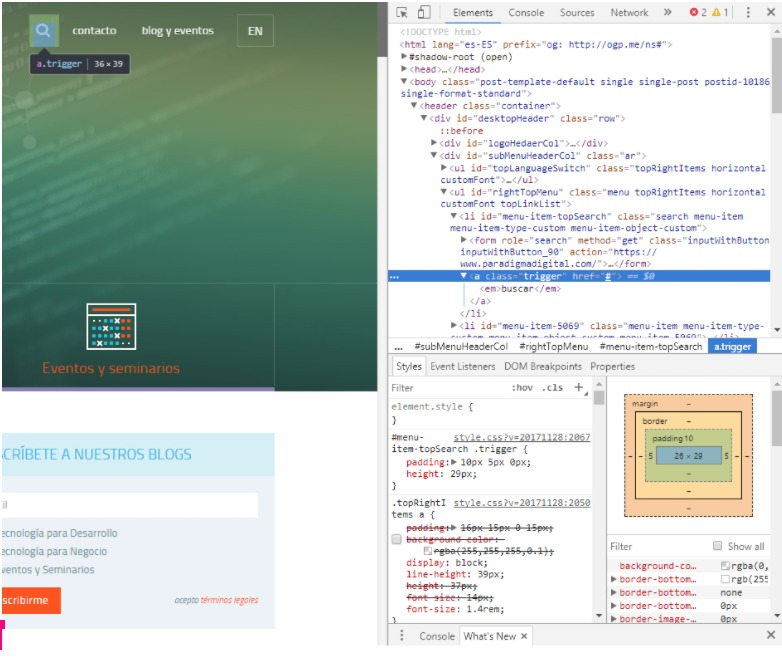
\includegraphics[width=200px]{./images/img1.jpg}
		\caption{Perspectivas del Cuadro de Mando Integrador}
	\end{center}
\end{figure}

Como podemos ver en la imagen anterior, la lupa es el siguiente elemento: <a class=”trigger” href=”#”>
Para la automatización es necesario identificar el elemento de manera unívoca. Para asegurarnos de que el elemento “a” con class “trigger” es el único elemento con estas propiedades, vamos a situarnos en la consola de Chrome e introducimos la siguiente función: $(“a.trigger”).
Como podemos ver en la documentación de la consola de Chrome $ es un alias de la función document.querySelectorAll().

\begin{figure}[H]
	\begin{center}
		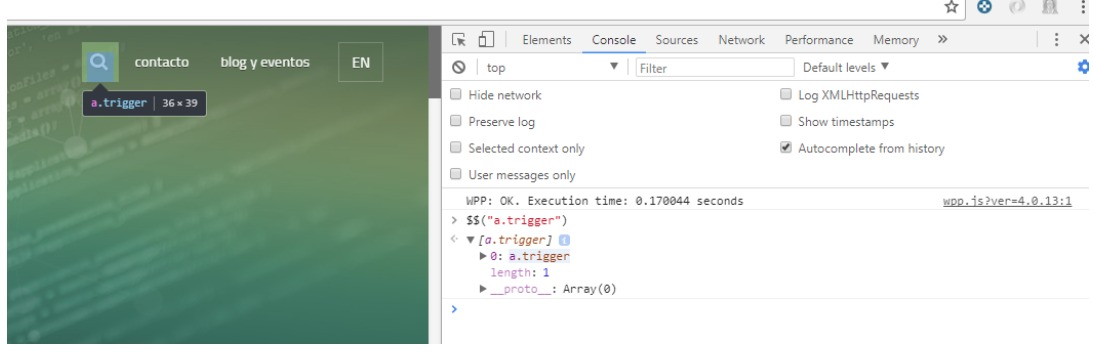
\includegraphics[width=200px]{./images/img2.jpg}
		\caption{}
	\end{center}
\end{figure}

Como podemos ver en la consola de Chrome, nos está indicando que en esta página solo hay un elemento “a” con el class “trigger”. Por lo que podemos concluir que el identificador CSS para el elemento de la lupa sería “a.trigger”.
Una vez que sabemos cómo buscar y obtener los identificadores de los elementos, vamos a explicar las principales funciones que se utilizan en el ejemplo.

FUNCIONES DE CYPRESS UTILIZADAS EN LOS EJEMPLOS

En el primer ejemplo que veremos a continuación, se utilizan las siguientes funciones:

\begin{enumerate} % Inicia enumeraci�n
	\item \textbf{}visit: redirige a Chrome a la url que se le pasa por parámetro.
	\item \textbf{}get: obtiene un elemento por el identificador que le pasemos, para realizar acciones sobre él. Como hemos explicado en el apartado anterior, todos los identificadores que pasemos será obtenidos del CSS.
	\item \textbf{}children: nos permite obtener un elemento que pasamos por parámetro, que desciende del elemento que hemos obtenido con la función get.
	\item \textbf{}click: realiza un click sobre el elemento que hayamos obtenido con la función get.
	\item \textbf{}type: escribe sobre el elemento obtenido un texto que pasamos por parámetro. Por ejemplo, usamos esta función para elementos input donde queremos introducir un texto.
	
	\item \textbf{}submit: permite enviar el contenido del formulario.
	
\end{enumerate}

A todas las funciones se les puede pasar un json con el elemento timeout. Este elemento nos permite incluir un tiempo que nos ayudará a esperar a que el elemento termine de cargar en la página.
Si no se incluye, Cypress intenta obtener los primeros elementos tras un visit y es muy probable que no dé tiempo a cargar el elemento o que no se haya cargado totalmente la estructura de la página.
Vamos a ejecutar un test que se encuentra en el fichero poc_cypress.js.

EJEMPLO

En este ejemplo vamos a realizar una prueba automática que acceda a mi anterior post, que compruebe que el autor es “Nicolás Cordero” y que realice una búsqueda por la cadena de texto chai-HTTP para encontrar el post que he escrito.
Como podemos ver en el ejemplo, utilizamos Mocha para realizar el test y Chai como librería de aserciones.

\begin{figure}[H]
	\begin{center}
		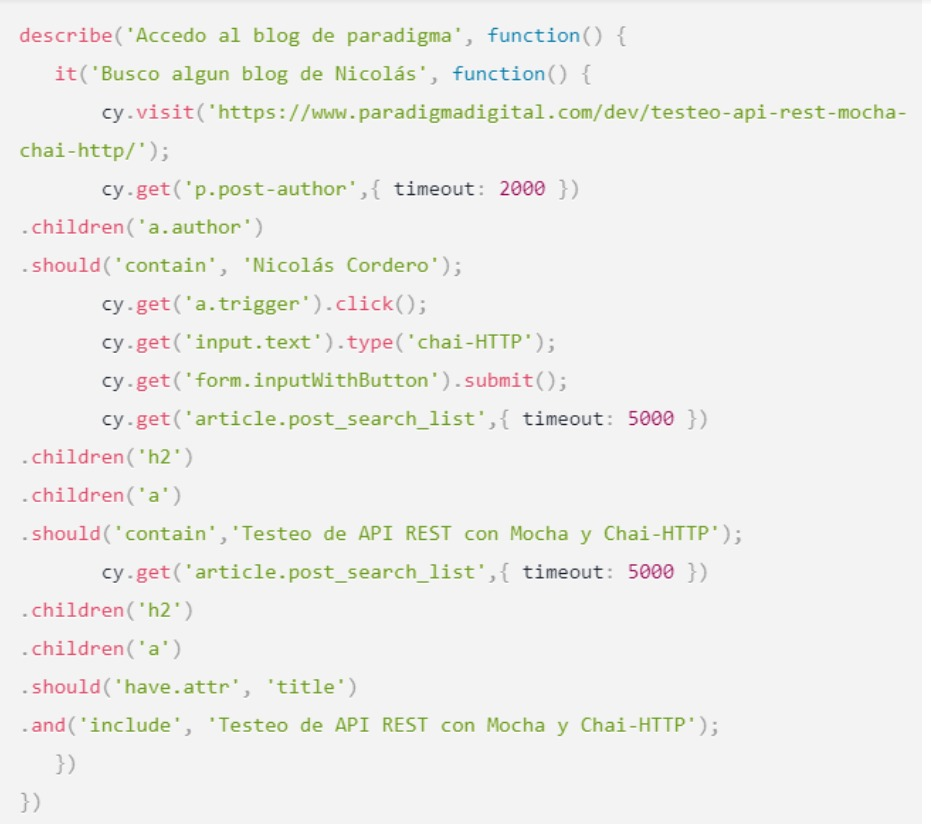
\includegraphics[width=200px]{./images/img3.jpg}
		\caption{}
	\end{center}
\end{figure}
En este ejemplo podemos observar que hemos pasado la variable timeout a ciertas funciones get, lo cual nos permite indicar un tiempo máximo que debe esperar hasta que el elemento ha sido cargado en la página.
Cypress, junto con la librería de aserciones Chai, nos permite realizar comprobaciones más completas de los elementos de una manera muy simple.
Por ejemplo, permite comprobar si el elemento dispone de algún atributo o si ese atributo o el elemento en cuestión contiene algún texto. En este ejemplo hemos usado:

\begin{enumerate} % Inicia enumeraci�n
	\item \textbf{}contains: para indicar el contenido del elemento.
	\item \textbf{}have.attr: para indicar que el elemento tiene un atributo en concreto.
	\item \textbf{}include: para indicar que el atributo de un elemento incluye un texto.
		
\end{enumerate}

POSTMAN

Postman es una herramienta que se utiliza, sobre todo, para el testing de API REST, aunque también admite otras funcionalidades que se salen de lo que engloba el testing de este tipo de sistemas.
Gracias a esta herramienta, además de testear, consumir y depurar API REST, podremos monitorizarlas, escribir pruebas automatizadas para ellas, documentarlas, mockearlas, simularlas, etc.
Quizás sea una de las herramientas más utilizadas para hacer testing exploratorio de este tipo de sistemas. Puede que no sea la mejor forma de escribir pruebas automatizada, pero sin duda es una de las más favorables para equipos con poca experiencia en programación, y sobre todo para hacer testing de todo tipo en general de API REST.
Es importante destacar también que, aunque no sea una de las herramientas más famosas para documentar API REST, genera una documentación bastante interesante y bastante atractiva, con ejemplos y snippets de código, de forma que hace que sea muy fácil de entender cómo funciona una API determinada.

CARACTERÍSTICAS PRINCIPALES :

\begin{enumerate} % Inicia enumeraci�n
	\item \textbf{}Permite la colaboración entre miembros del equipo.
	\item \textbf{}Tiene una interfaz más intuitiva y atractiva.
	\item \textbf{}Posee extensión para Google Chrome,  por lo tanto no es necesario instalar la aplicación de escritorio.
		\item \textbf{}Como ya mencionamos en la descripción, tiene una opción muy interesante, que son las colecciones, que funciona básicamente como una base de datos de peticiones.
	\item \textbf{}Es extensible y se puede integrar con otras herramientas, por ejemplo ejecutando las suites de prueba desde un motor  de CI/CD.
	\item \textbf{}Permite agregar scripts en lenguaje Javascript para agregar validaciones, configurar y/o automatizar pruebas (esto se realiza directamente en la petición).
	
	
	
\end{enumerate}

EJEMPLO : 
En este ejemplo se simulará la información de cripto divisas 
Código en Java

\begin{figure}[H]
	\begin{center}
		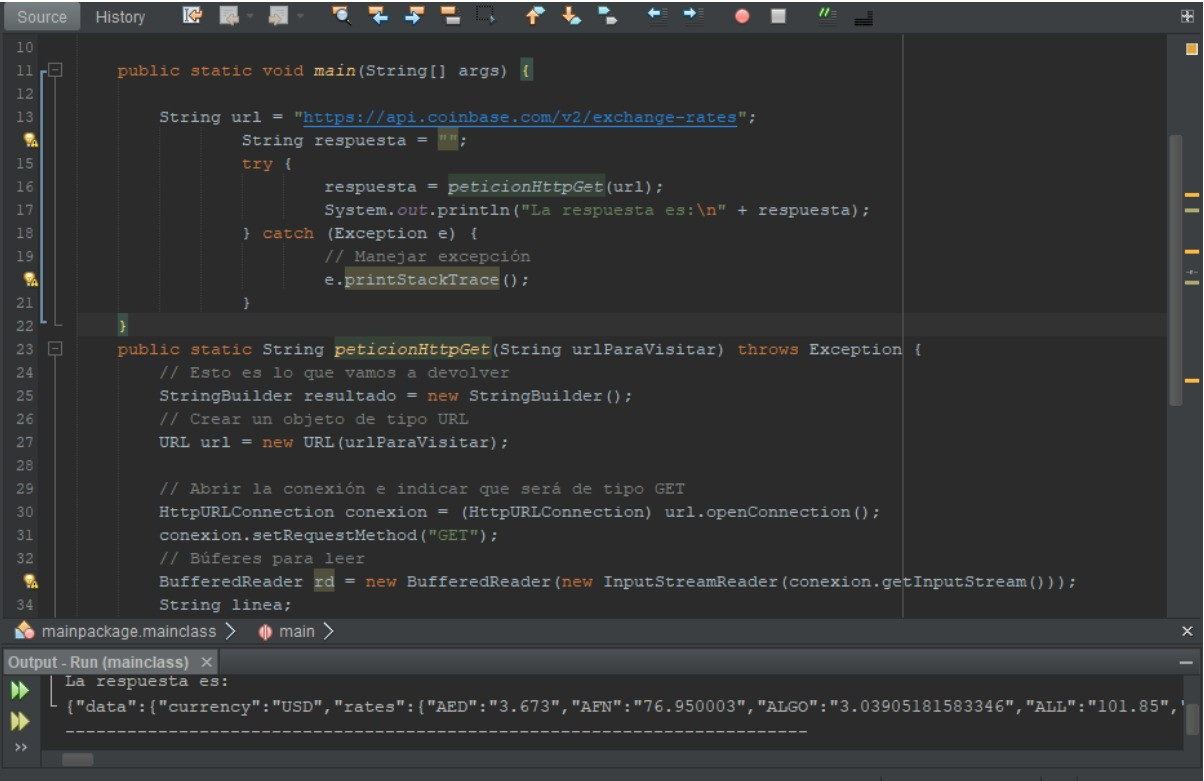
\includegraphics[width=200px]{./images/img4.jpg}
		\caption{}
	\end{center}
\end{figure}

Se ingresa la URL en Postman para así recibir un texto en formato JSON

\begin{figure}[H]
	\begin{center}
		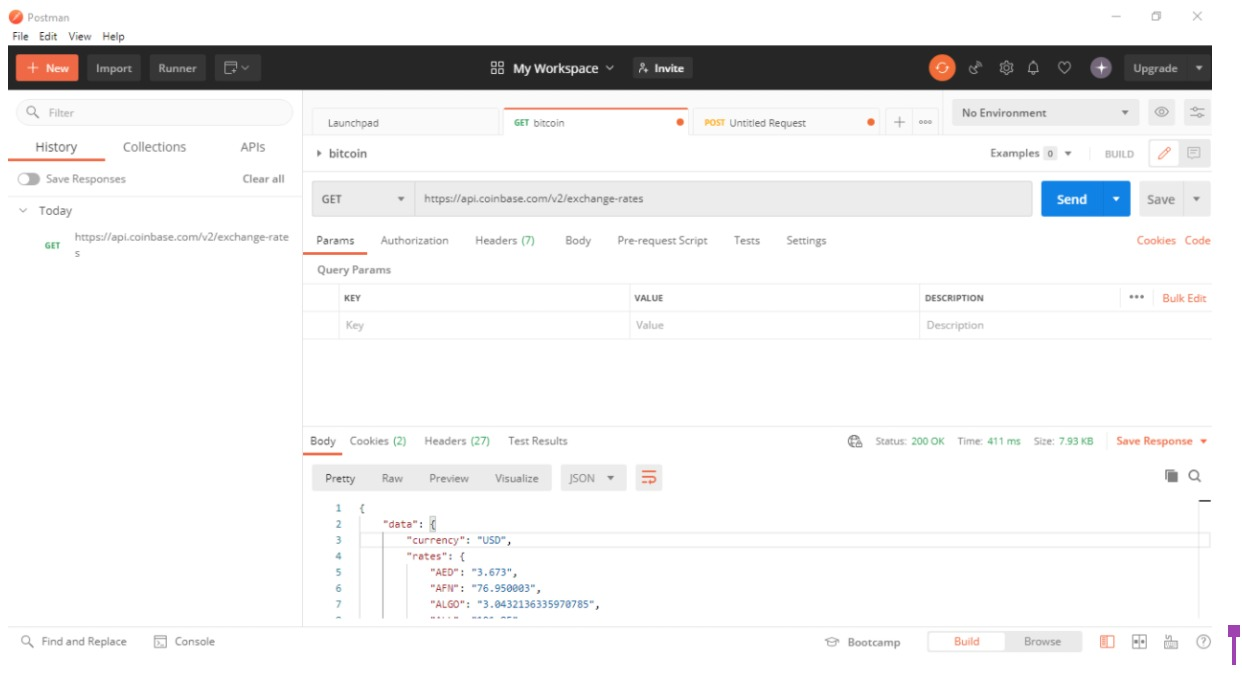
\includegraphics[width=200px]{./images/img5.jpg}
		\caption{}
	\end{center}
\end{figure}



%Colocar una imagen
\begin{figure}[H]
\begin{center}
  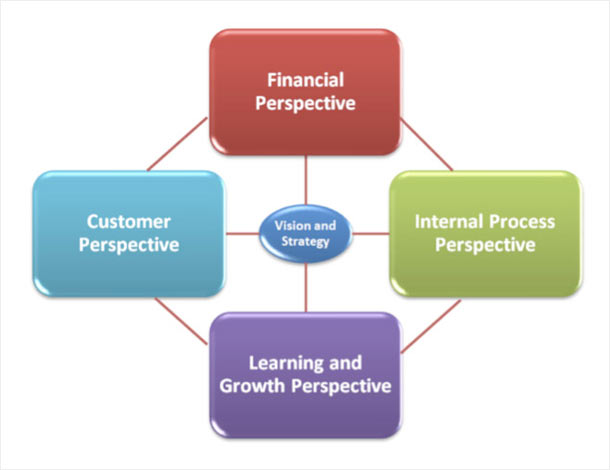
\includegraphics[width=200px]{./images/bsc1.jpg}
  \caption{Perspectivas del Cuadro de Mando Integrador}
\end{center}
\end{figure}



\section{Conclusiones}
Es útil para el Ingeniero de Pruebas conocer cómo se entrelazan su herramienta de pruebas automatizadas y el framework que utiliza para así comprender mejor los conceptos a utilizar y cómo la herramienta implementa dichos conceptos.

\section{Recomendaciones}
Se recomienda  conocer cuáles son las distintas opciones de frameworks que existen en la actualidad para así realizar una decisión informada sobre cuál o cuáles son los frameworks más adecuados para su proyecto y también para realizar su trabajo de la forma más rápida y eficiente posible.
% Bibliografía.
%-----------------------------------------------------------------
% para agregar más referencias es necesario abrir el archivo : biblio/bibliografia.bib
% Compilar las referencias desde la línea de comandos o terminal:
% $ latex PaternoMatenoN_plantillatarea
% $ bibtex PaternoMatenoN_plantillatarea
% $ latex PaternoMatenoN_plantillatarea
% $ latex PaternoMatenoN_plantillatarea
%-----------------------------------------------------------------

\bibliography{biblio/bibliografia.bib}
\setlength{\parindent}{-0.2in}
\setlength{\leftskip}{0.2in}
\setlength{\parskip}{8pt}
\vspace*{-0.2in}
\noindent
\bibliographystyle{apacite}
Suarez Fernando. (2020). Frameworks de QA en 2020. 10/05/2020, de Qantum 

Aldaine Alice. (2018). Top 10 API Testing Tools in 2020. 28/05, de médium

Cordero Nicolás. (2018). Cypress, un framework de pruebas todo en uno. 15/05, de Paradigma 

Briceño Luis. (2017). 22 curiosidades antes de usar Cypress.io. 21/07, de GFourmis 

Toledo Federico. (2020). API testing con Postman y SoapUI. 19/08, de Federico 

Postman. (2014). Postman. 24/10, de Capterra 
López Alejandro. (2019). 

Ventajas de Postman sobre otros entornos similares. 09/06, de OpenWebinars

Parada Miguel. (2018). Framework Abiertos para testing Automation. 25/03, de openexpo Europe 



\end{document}
